\documentclass[11pt]{article}

\usepackage[margin=1in]{geometry}
\usepackage{amsmath,amssymb}
\usepackage{booktabs}
\usepackage{graphicx}
\usepackage{microtype}
\usepackage{hyperref}
\usepackage{enumitem}
\hypersetup{colorlinks=true,allcolors=blue}
\setlist{nosep}

\title{Auditing Addition-Circuit Interpretations in GPT-2 Small: Behavioral Baselines and an Equal-Operand Preference}
\author{Anay Katiyar\\\small Independent Researcher}
\date{}

\begin{document}
\maketitle

\begin{abstract}
Does GPT-2 Small use an identifiable circuit to perform simple decimal addition, or can its apparent arithmetic behavior be explained by prompt and token-level preferences? We audit saved behavioral, attribution, intervention, and prompt-comparison results for GPT-2 Small (124M parameters) on short addition prompts. In a held-out zero-shot cohort, top-1 accuracy is 2/32, compared with 8/32 for the best constant guess. In a 79-cell prompt grid, the sign of a neighbor-averaged target logit contrast agrees with target parity in 68/79 cells, but agreement differs sharply across target ranges. A matched scan of seven even target sums finds a descriptive equal-operand advantage of +0.247 (reported SE 0.102), positive at six targets. Correcting final-LayerNorm scaling and separating unembedding bias narrows earlier component interpretations; candidate-component screens remain exploratory and do not establish a circuit. Corpus-proxy outputs are incomplete and do not report an association test. The evidence supports a target-dependent prompt-level preference, not a general addition mechanism or a claim that arithmetic representations are absent.
\end{abstract}

\section{Introduction}

Mechanistic interpretability seeks explanations of model behavior in terms of internal representations and computations, rather than correlations between inputs and outputs alone \cite{elhage2021framework}. GPT-2 is an autoregressive language model trained on next-token prediction \cite{radford2019gpt2}; arithmetic is an attractive test case because the intended operation is explicit, but a model's preference for a correct answer token is not by itself evidence that it carried out the operation.

The closest comparison in model and method is the study of greater-than prediction in pretrained GPT-2 Small by Hanna et al. \cite{hanna2023greater}. They identify and test a circuit for comparing year-like values. Their task and positive circuit result motivate asking whether similarly controlled evidence supports a circuit for decimal addition; they do not establish that it does. Other influential addition studies analyze small transformers trained on modular addition. Nanda et al. reverse-engineer a Fourier-based algorithm in a grokked model, while Zhong et al. show that closely related training setups can yield distinct algorithms \cite{nanda2023progress,zhong2023clock}. These are important demonstrations of what mechanistic evidence can establish in controlled trained models, but they differ from a pretrained language model completing familiar text strings. Ye et al. study hidden processes in models trained on synthetic grade-school math, another distinct training and task setting \cite{ye2024physics}.

This work audits a set of GPT-2 Small probes on prompts such as \texttt{3 + 5 =}. The initial hypothesis concerned a general addition-specific circuit. Behavioral baselines, attribution corrections, and intervention controls narrowed that interpretation. A target-dependent preference for equal-operand prompts remained in a seven-target scan, so we examine it as a descriptive behavioral effect and a candidate for future causal testing.

Our contribution is an evidence-bounded report of these probes and their corrections. We do not claim to identify an addition algorithm. In particular, the available data support neither a general circuit account nor the stronger claim that GPT-2 Small has no arithmetic-related representations.

\section{Study scope and related work}

\paragraph{Pretrained mathematical behavior.} Hanna et al. examine a greater-than task in pretrained GPT-2 Small and validate a circuit across related contexts \cite{hanna2023greater}. This is the nearest precedent by model family and mechanistic method. The present study differs in the behavior (decimal addition rather than year-span comparison), and it does not meet the same standard of circuit identification or generalization.

\paragraph{Addition circuits in trained models.} Nanda et al. study small transformers trained on modular addition and use activation, weight, and intervention analyses to validate a learned Fourier algorithm \cite{nanda2023progress}. Zhong et al. show that learned modular-addition solutions vary with architecture and training conditions \cite{zhong2023clock}. Lee et al. study how training data and formats affect arithmetic learning in small transformers \cite{lee2024teaching}. These studies motivate testing the algorithm actually learned rather than assuming that a task name specifies a mechanism. Their synthetic training regimes, modular arithmetic, and model behaviors differ from the pretrained decimal-completion setting here.

\paragraph{Other mathematical and circuit methods.} Ye et al. analyze internal processes in synthetic grade-school math settings, including GPT-2-family models trained on generated data \cite{ye2024physics}. Their results motivate separating behavioral competence from internal-process evidence, but do not transfer to the present prompts. Circuit evaluation work on indirect-object identification and automated circuit discovery motivates explicit behavioral metrics and causal validation \cite{wang2023ioi,conmy2023acdc}. Those papers supply methodological context only; all measurements below come from this project's saved artifacts.

\section{Methods}

\subsection{Model, prompts, and saved records}

The reported model is GPT-2 Small (124M parameters). Prompts use short textual arithmetic forms, principally \texttt{a + b =}. The repository preserves a full-record notebook with saved outputs, a 79-row addition grid, a 39-row digit-addition double/control score file, aggregate format and operator summaries, and an artifact manifest. The notebook was not independently rerun for this manuscript. We therefore distinguish saved-run observations from independent reproduction.

The behavioral report includes an all-pairs zero-shot cohort ($N=36$), a separate held-out zero-shot cohort ($N=32$), and a held-out few-shot cohort ($N=32$). These are distinct evaluations and are not pooled. The dense equal-operand scan covers the seven even target sums $T\in\{4,6,8,10,12,14,16\}$. For each target, it compares the single double prompt $(T/2)+(T/2)$ with the available ordered, unequal, single-digit splits that sum to $T$.

\subsection{Behavioral metrics}

Behavioral competence is measured by full-vocabulary top-1 accuracy and compared with a constant-guess baseline on the same held-out cohort. For prompt $p$ and target token $T$, the neighbor-averaged logit contrast is
\begin{equation}
S(p,T)=\ell_T(p)-\frac{\ell_{T-1}(p)+\ell_{T+1}(p)}{2},
\label{eq:score}
\end{equation}
where $\ell_j(p)$ is the next-token logit for the leading-space answer token corresponding to $j$. This score measures relative logit preference among the target and its two neighboring values; it is not a measure of exact-answer probability or proof of arithmetic computation.

For each even target $T$, the equal-operand advantage is
\begin{equation}
A_T=S(p_{d,d},T)-\frac{1}{|C_T|}\sum_{(a,b)\in C_T}S(p_{a,b},T),\qquad d=T/2,
\label{eq:adv}
\end{equation}
where $p_{a,b}$ is the prompt \texttt{a + b =} and $C_T$ contains the evaluated ordered unequal splits with $a+b=T$. The reported mean and standard error summarize these seven target-level advantages. With one double prompt per target and only seven target values, the summary is treated descriptively; the normalized $A_T/\mathrm{SD}$ quantities are not significance tests.

The addition-grid analysis records whether the sign of the measured symmetric logit contrast matches target parity. Grid cells share target values and are not independent observations.

\subsection{Attribution and intervention audits}

The saved attribution analyses project residual components onto a target-versus-foil unembedding direction. The audit corrected an earlier calculation by applying final LayerNorm scaling to the residual decomposition before projection and by separately including the unembedding bias term when reconstructing the measured logit contrast. These corrections change the interpretation of selected prompts; attribution alone does not establish necessity or sufficiency.

Intervention summaries compare zero-ablation with mean-ablation and report candidate-component screens with false-discovery-rate-adjusted $q$ values. A separate operator-position patching experiment lacked a corrupt-baseline anchor, so it cannot establish that operator binding was falsified. We keep that experiment distinct from the aggregate operator-string comparisons.

\subsection{Format, operator, and corpus comparisons}

Format summaries compare digit--digit, digit--word, and word--word prompts. Prompt-level formatted control scores are not available, so the pooled format dispersions cannot be independently recomputed. Operator and connector summaries compare strings such as \texttt{+}, \texttt{-}, \texttt{*}, \texttt{and}, and \texttt{then}. For non-addition strings, the analysis still scores the arithmetic sum token; these comparisons therefore test the persistence of a logit preference across strings, not whether the model correctly performs subtraction or multiplication.

The corpus audit uses Infini-gram counts from the Dolma v1.7 index \texttt{v4\_dolma-v1\_7\_llama} as a proxy for possible textual co-occurrence. It queries exact double strings and matched unequal-operand controls. The raw collector intentionally applies no eligibility floor and computes no correlation. Dolma is not GPT-2's exact training corpus.

\section{Results}

\subsection{The tested cohorts do not show reliable exact-answer performance}

Full-vocabulary top-1 accuracy is 2/36 (5.56\%) on the all-pairs zero-shot cohort and 2/32 (6.25\%) on the held-out zero-shot cohort. On the held-out zero-shot set, the best constant guess scores 8/32 (25\%). Held-out few-shot accuracy is also 2/32. These cohort-specific results do not establish that GPT-2 Small lacks all arithmetic-related computation; they show that the evaluated prompt sets do not support a claim of reliable exact-answer addition above the simple held-out baseline.

\subsection{Parity agreement varies across the addition grid}

In the committed 79-cell grid, target parity predicts the sign of the measured logit contrast in 68/79 cells. Agreement is 63/64 for sums $\leq 13$ and 5/15 for sums $\geq 14$. Because cells share target sums and have different prompt compositions, these fractions are descriptive rather than independent-trial estimates. The pattern is not uniform across the tested range.

\begin{figure}[t]
\centering
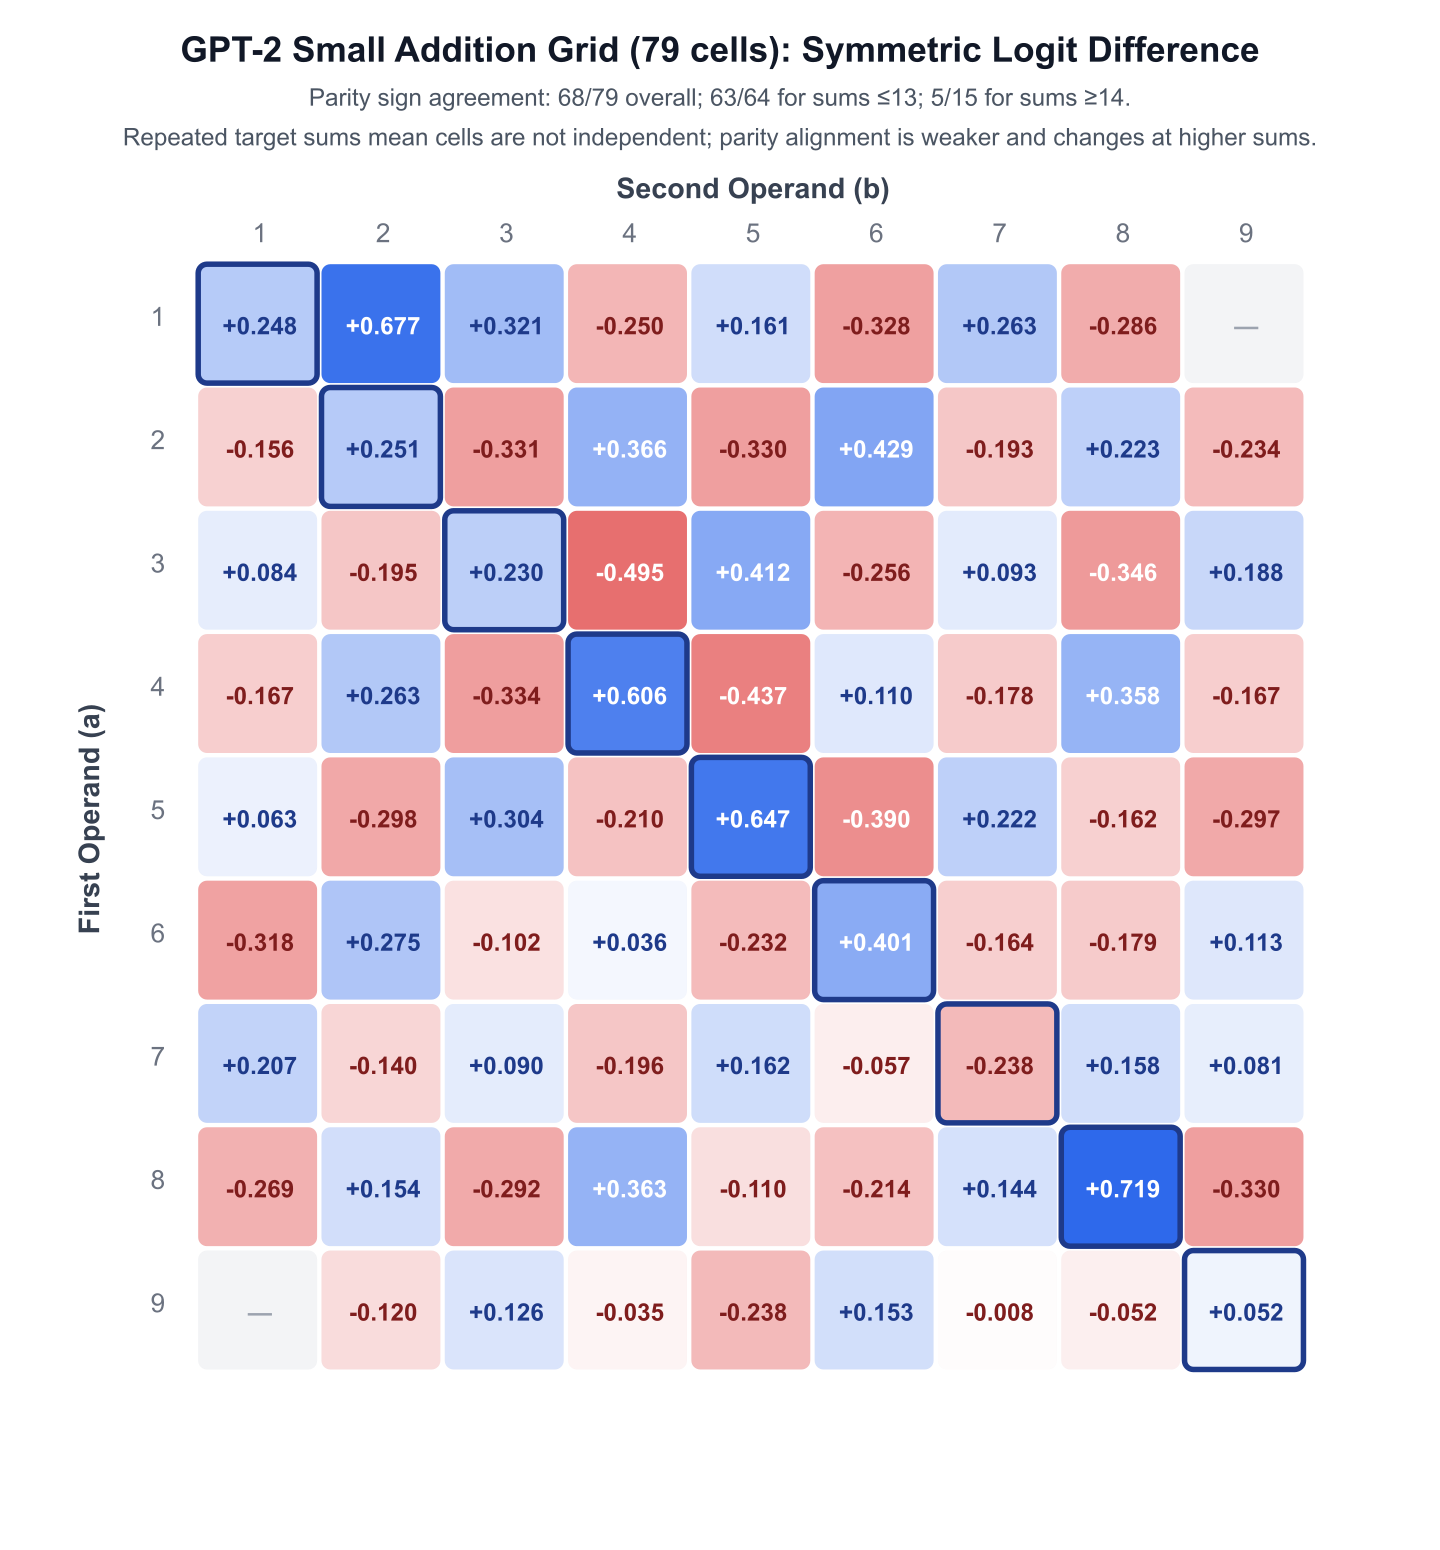
\includegraphics[width=0.88\linewidth]{addition_grid_heatmap.png}
\caption{Addition-grid symmetric logit differences across the 79 committed prompt pairs. The grid shows target-dependent structure; cells sharing a target are not independent observations. Figure regenerated from the committed grid.}
\label{fig:addition-grid}
\end{figure}

\subsection{Attribution corrections narrow component interpretations}

For the saved \texttt{3 + 5 =} comparison, corrected residual-component DLA sums to $+0.4658$ and the reported unembedding-bias contrast is $+0.1782$; together they reconstruct $+0.6440$, against a measured logit difference of $+0.6443$. The small discrepancy is retained as reported. In a separate few-shot comparison on \texttt{158 + 274 =}, the dynamic contribution is $+0.8382$ and the bias term is $-1.0303$, against a reported logit difference of $-0.1920$. That contrast compares the leading-space tokens \texttt{8} and \texttt{1}, although the arithmetic answer is 432; it is a token-contrast identity, not evidence that the model computed 8 and was overridden.

Zero-ablation changed the residual-stream scale in the reported prompt. Under mean-ablation across reference prompts, the reported L11H0 shift is $+0.0013$; joint ablation of L11H0 and MLP10 gives $+0.8127$ against an additive prediction of $+0.8131$ on that prompt. These results do not support the earlier suppressor and non-additivity interpretations for the tested prompt and intervention.

\subsection{A target-dependent equal-operand preference remains}

The 39-row digit--digit scan reports the following target-level summaries:

\begin{center}
\small
\begin{tabular}{rrrrrr}
\toprule
Target $T$ & Double score & Control mean & Advantage $A_T$ & $A_T/\mathrm{SD}$ & Controls \\
\midrule
4  & $+0.251$ & $+0.203$ & $+0.049$ & $+0.29$ & 2 \\
6  & $+0.230$ & $+0.213$ & $+0.017$ & $+0.13$ & 4 \\
8  & $+0.606$ & $+0.315$ & $+0.291$ & $+3.31$ & 6 \\
10 & $+0.647$ & $+0.113$ & $+0.535$ & $+9.54$ & 8 \\
12 & $+0.401$ & $+0.236$ & $+0.165$ & $+1.63$ & 6 \\
14 & $-0.238$ & $-0.232$ & $-0.006$ & $-0.12$ & 4 \\
16 & $+0.719$ & $+0.037$ & $+0.682$ & $+10.83$ & 2 \\
\bottomrule
\end{tabular}
\end{center}

The reported mean advantage is $+0.247$ (SE $0.102$), with positive advantages at six of seven target sums. The target-level pattern is heterogeneous: effects are largest at some sums and near zero at others. The $A_T/\mathrm{SD}$ column is descriptive and must not be read as a $t$ statistic or significance test. The result is a preference in the tested prompt and scoring setup; it does not identify a mechanism.

Format-level summaries report mean advantages of $+0.418$ for digit--digit, $+0.750$ for digit--word, and $+1.349$ for word--word at targets 8, 10, 12, and 16. These are aggregate summaries without the prompt-level formatted controls required to recompute all pooled standard deviations. The presence of an advantage in digit--word prompts means literal repetition of the same written digit is not necessary in these displayed conditions; it does not exclude lexical-equivalence, template, or familiarity explanations.

Across the reported operator and connector strings, aggregate advantages are present, but the task is not semantically matched: the same sum token is scored under strings for addition, subtraction, multiplication, and connectives. The largest raw advantage is reported under \texttt{then} ($+0.549$), while the largest normalized ratio is reported under subtraction (6.15). These summaries are descriptive, lack prompt-level scores, and do not establish operator-insensitive arithmetic.

\begin{figure}[t]
\centering
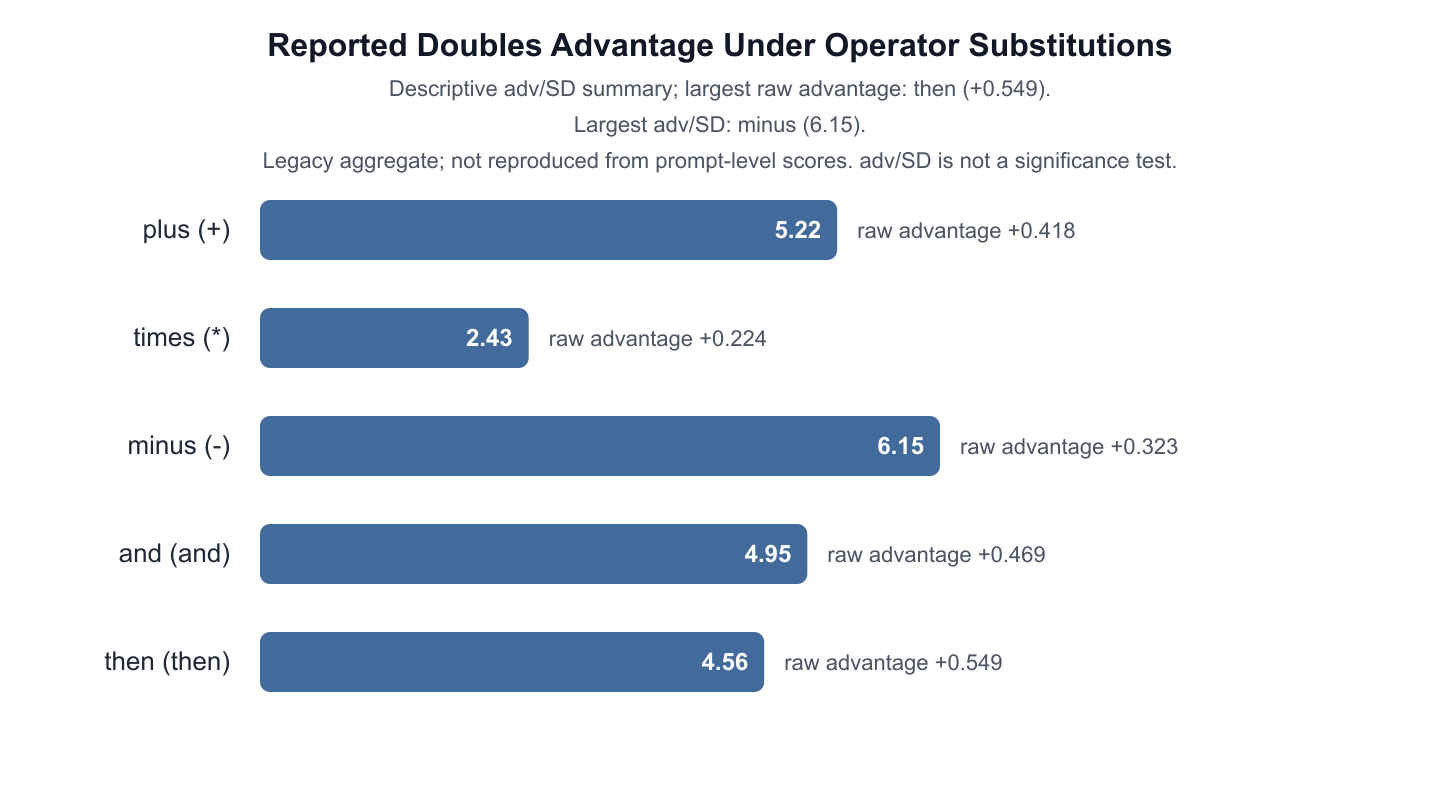
\includegraphics[width=0.96\linewidth]{operator_swap_heatmap.png}
\caption{Reported normalized advantage-to-control-standard-deviation ratios for operator and connector strings. This is an aggregate descriptive summary without prompt-level scores; the same arithmetic-sum token is scored in every condition, so it is not a test that the model computes each operation.}
\label{fig:operator-summary}
\end{figure}

\subsection{Candidate-component screens do not establish a circuit}

The saved notebook identifies \texttt{10\_mlp\_out}, L9H9, and L10H2 as candidates for further study. The component DLA screen reports $q_{\mathrm{FDR}}=0.513$ and the two-sided mean-ablation screen reports $q_{\mathrm{FDR}}=0.150$; neither passes the stated 0.05 threshold. Transfer is mixed, targets were not a blind holdout, and filler prompts also show effects. The aggregate removal-fraction calculation also has a documented discrepancy. These screens do not establish necessity, sufficiency, minimality, or a validated addition circuit.

\subsection{Corpus-frequency relationship remains unresolved}

The repository notebook's raw collector output records 79 query attempts and no failed attempts. A later saved collector output records 80 attempts and one failure. Both display the same seven-target summary, but per-attempt response logs are not available to identify the additional attempt. Neither raw collector reports a correlation or applies an eligibility floor. The data therefore do not establish whether corpus co-occurrence tracks the equal-operand preference. The relationship also cannot be interpreted as GPT-2 training exposure because Dolma is only a proxy.

\section{Discussion}

The study began with a possible addition-circuit interpretation. The behavioral baseline does not demonstrate reliable exact-answer performance on the tested cohorts. The parity grid shows structured but range-dependent logit preferences. Attribution and intervention audits narrow several component-level explanations. Against this background, the equal-operand scan provides a specific, reproducible prompt-level pattern in the committed score file: a positive mean advantage across seven target sums, with substantial target variation. The cause of this pattern has not been identified.

This evidence differs from Hanna et al.'s positive greater-than circuit account: the model family is shared, but the task differs and the present candidate screens do not validate a circuit \cite{hanna2023greater}. It also differs from the modular-addition literature, where models are trained directly on a formal arithmetic task and the learned algorithm is supported by weight, activation, and intervention evidence \cite{nanda2023progress,zhong2023clock}. The current results are best understood as a cautious audit of arithmetic-like behavior in a pretrained text model, not as a failed replication of those studies or evidence against their findings.

The most direct follow-up would test whether the equal-operand preference survives independent target selection, prompt-level token and format controls, and preregistered causal interventions. Such a study should retain per-prompt outputs, use matched clean and corrupted baselines, reserve held-out targets, and evaluate both necessity and restoration. A single-operand control and semantically appropriate scoring for operator variants are also needed before interpreting these patterns as arithmetic computations.

\section{Limitations}

The study examines one model, a narrow set of short prompts, and a small number of target sums. Several cohort definitions and few-shot prefixes differ and are not pooled. Some reported values are saved notebook outputs rather than outputs independently regenerated from a clean environment. Formatted and operator-specific prompt-level scores, corpus API responses, and some intermediate outputs are absent from the repository. The corpus collector does not perform an association test, and one later run's attempt count differs from the repository notebook output. The single-operand comparison remains untested. Candidate-component results are exploratory and cannot support a circuit claim.

The equal-operand advantage is based on one double prompt per target and a small target set; the reported SE is descriptive and does not convert target sums into independent replications. The operator comparisons score the arithmetic-sum token even when the prompt string denotes a different operation. The corpus proxy is not the model's training corpus. These limitations constrain both mechanistic and generalization claims.

\section{Conclusion}

On the evaluated prompts, the evidence does not establish a general addition-specific circuit in GPT-2 Small. Auditing the measurement pipeline weakened several earlier component interpretations. A target-dependent equal-operand preference remains in the saved prompt scores, but the available interventions do not explain it. The appropriate conclusion is neither that GPT-2 Small has been shown to calculate addition through a specific circuit nor that it lacks arithmetic-related computation. The surviving result motivates a more controlled causal study.

\section*{Data and code availability}

The research notebook, committed score tables, audit trail, and scripts are available at \url{https://github.com/anaykatiyar-lang/mechanistic_interpretability}. The notebook contains saved outputs and was not independently rerun for this manuscript. The manifest identifies generated outputs and per-prompt records that are not available in the repository. The later corpus collector output is described in the audit record; its raw per-attempt log was not archived.

\section*{AI assistance disclosure}

Claude Sonnet 5.5, ChatGPT, and Gemini 3.1 Pro assisted with literature exploration, code, and writing. Their suggestions were treated as prompts for review, not as evidence. The author checked claims against available records and is responsible for the experiments, data, analysis, and final manuscript. Some results cannot be independently regenerated from the available materials.

\begin{thebibliography}{99}

\bibitem{conmy2023acdc}
A.~Conmy, A.~N. Mavor-Parker, A.~Rachubinski, A.~Nanda, and A.~Thomas.
\newblock Towards automated circuit discovery for mechanistic interpretability.
\newblock In \emph{Advances in Neural Information Processing Systems}, 2023.
\newblock \url{https://arxiv.org/abs/2304.14997}.

\bibitem{elhage2021framework}
N.~Elhage et~al.
\newblock A mathematical framework for transformer circuits.
\newblock \emph{Transformer Circuits Thread}, 2021.
\newblock \url{https://transformer-circuits.pub/2021/framework/index.html}.

\bibitem{hanna2023greater}
M.~Hanna, O.~Liu, and A.~Variengien.
\newblock How does GPT-2 compute greater-than? Interpreting mathematical abilities in a pre-trained language model.
\newblock In \emph{Advances in Neural Information Processing Systems}, 2023.
\newblock \url{https://arxiv.org/abs/2305.00586}.

\bibitem{lee2024teaching}
N.~Lee, K.~Sreenivasan, J.~D. Lee, K.~Lee, and D.~Papailiopoulos.
\newblock Teaching arithmetic to small transformers.
\newblock In \emph{International Conference on Learning Representations}, 2024.
\newblock \url{https://arxiv.org/abs/2307.03381}.

\bibitem{nanda2023progress}
N.~Nanda, L.~Chan, T.~Lieberum, J.~Smith, and J.~Steinhardt.
\newblock Progress measures for grokking via mechanistic interpretability.
\newblock In \emph{International Conference on Learning Representations}, 2023.
\newblock \url{https://arxiv.org/abs/2301.05217}.

\bibitem{radford2019gpt2}
A.~Radford et~al.
\newblock Language models are unsupervised multitask learners.
\newblock OpenAI technical report, 2019.
\newblock \url{https://cdn.openai.com/better-language-models/language_models_are_unsupervised_multitask_learners.pdf}.

\bibitem{wang2023ioi}
K.~Wang, A.~Variengien, A.~Conmy, B.~Shlegeris, and J.~Steinhardt.
\newblock Interpretability in the wild: A circuit for indirect object identification in GPT-2 small.
\newblock In \emph{International Conference on Learning Representations}, 2023.
\newblock \url{https://arxiv.org/abs/2211.00593}.

\bibitem{ye2024physics}
T.~Ye, Z.~Xu, Y.~Li, and Z.~Allen-Zhu.
\newblock Physics of language models: Part 2.1, grade-school math and the hidden reasoning process.
\newblock arXiv:2407.20311, 2024.
\newblock \url{https://arxiv.org/abs/2407.20311}.

\bibitem{zhong2023clock}
Z.~Zhong, Z.~Liu, M.~Tegmark, and J.~Andreas.
\newblock The clock and the pizza: Two stories in mechanistic explanation of neural networks.
\newblock In \emph{Advances in Neural Information Processing Systems}, 2023.
\newblock \url{https://arxiv.org/abs/2306.17844}.

\end{thebibliography}

\end{document}
